\documentclass[12pt,letterpaper]{article}
\usepackage{fullpage, lastpage, enumerate, fancyhdr, titlesec}
\usepackage[top=2cm, bottom=4.5cm, left=2.5cm, right=2.5cm]{geometry}
\usepackage{amsmath,amsthm,amsfonts,amssymb,amscd}
\usepackage{mathrsfs, xcolor, graphicx, subcaption, siunitx}
\usepackage{hyperref}
\graphicspath{{./images}}

\hypersetup{%
  colorlinks=true,
  linkcolor=blue,
  linkbordercolor={0 0 1}
}

\setlength{\parindent}{0.0in}
\setlength{\parskip}{0.05in}

\titleformat{\subsection}
  {\normalfont\normalsize\itshape}{\thesubsection}{1em}{}

\pagestyle{fancyplain}
\headheight 15pt
\fancyhf[FL]{Matthew Bernstein}
\fancyhf[HR]{\today}
\fancyhf[HL]{ISyE 7406 - Homework 2}
\fancyhf[FC]{}
\fancyhf[FR]{\thepage}
\headsep 1.5em

\title{ISYE 7406 - Homework 2}
\author{Matthew Bernstein}

\begin{document}
\fancypagestyle{plain}{
    \fancyhf{}
    \renewcommand{\headrulewidth}{0pt}
    \renewcommand{\footrulewidth}{0pt}
}
\maketitle
\section*{Introduction}

In this experiment, different methods of fitting and pruning linear regression models were tested. The dataset included 2 measures of bodyfat percentage as well as 16 other body measurements. In particular, we were trying to see if the body measurements had any predicitve power on the bodyfat percentage as calculated by the Brozek formula.

Eight models were fit using various feature selection and regularization techniques for a single train/test split of the data and then repeated in a 500 trial MonteCarlo cross validation routine. Accuracy for each model was assessed using mean squared error on the test set. 

\section*{Exploratory Data Analysis}

The data set contains 252 observations of 17 features and one response, \textit{brozek}. Most of the feautres are bodily measurements, such as chest circumference, or weight. 

Figure \ref{fig:cor} shows a correlation heatmap between all features and the response. There are a couple noticeable characteristics. First, \textit{brozek}, is a function of \textit{density}, as shown by the high negative correlation. Second, \textit{brozek} and \textit{siri} are extremely positively correlated since both are a measure of body fat with very similar formulas. Finally, there is almost no correlation between \textit{brozek} and \textit{free}. This is because \textit{free} is a function of \textit{brozek}. These 3 factors were dropped from further analysis since they were already explicitly related to the response variable. 

\begin{figure}[!htb]
  \centering
  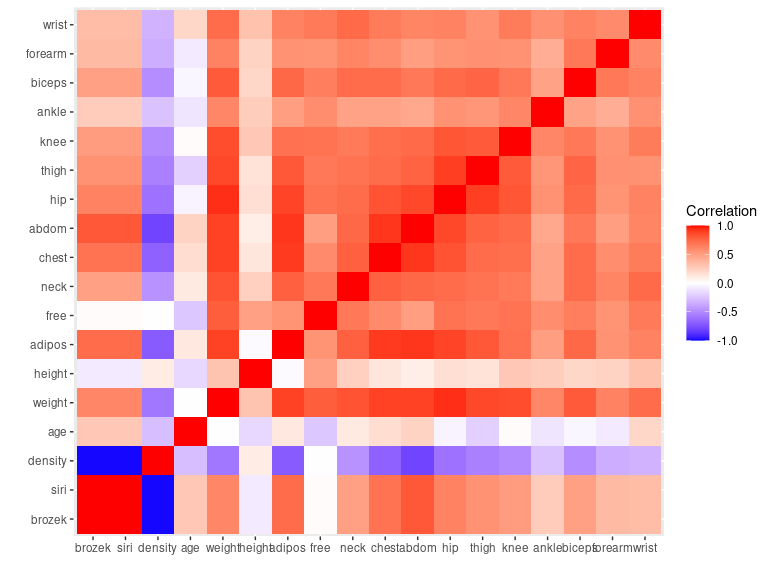
\includegraphics[width=0.6\textwidth]{cor_heatmap}
  \caption{Correlation heatmap}
  \label{fig:cor}
\end{figure}

\section*{Methodology}

Eight models were created from the data in order to understand the different types of Linear Regressions

\subsection*{Full Model}
A least squares linear model was fitted on all features, excluding \textit{siri}, \textit{density}, \textit{free} as noted above.

\subsection*{5 Best Feature Selection}
Two models were created by selecting the 5 best features and performing a regression against those. The first model was created by selecting the 5 features with the lowest p-scores in the full model. The second model was selected by performing an exhaustive search over all combinations of 5 features and selecting the combination with the lowest Mallow's Cp score. 

\subsection*{Stepwise Regression}
A model was created using a bi-directional stepwise regression. Beginning with an empty model, a single feature was added or removed and the AIC of the resulting model was calculated. This process was repeated until no changes to the model from the previous step improved upon the model. 

\subsection*{Ridge Regression}
A Ridge regression model was created using the full dataset. The $\lambda$ parameter was selected using a 5-fold cross validation minimizing the MSE of the validation set error

\subsection*{LASSO}
LASSO was used for feature selection by fitting the full feature set and then selecting the the features with non-zero coefficients. The $\lambda$ parameter was selected using a 5-fold cross validation minimizing the MSE of the validation set error. Once the reduced feature set was decided, a linear regression was fit on those features

\subsection*{PCA}
Principle Component Analysis dimension reduction was performed on the dataset to calculate a number of PCs equal to the number of features. Then $N$ PCs were selected to fit a linear regresion where $N$ is the number of PCs needed to explain at least 95\% of total variance in the dataset. 

\subsection*{PLS}
Partial Least Squares analysis was performed on the data set to calculate a set of components. 10-fold cross validation was used to select the optimal number of components for a linear regression by minimizing the MSE of the validation set.

\subsection*{MonteCarlo Cross Validation}
Each of the 8 models was then repeated in a 500 trial MonteCarlo cross validation with the test error saved and aggregated for each trial. 

\section*{Results}

Table \ref{tab:coef} shows the coefficients of the 8 models created. The full model and ridge regression both include all features. The two method of selcting the 5 "best" features selected almost the same set, with AIC prefering \textit{thigh}, while p-score selecting \textit{neck} instead.

\begin{table}
  \centering
  \scalebox{0.73}{
    \begin{tabular}[h]{|l||r|r|r|r|r|r|r|r|}
    \hline
      & Full & 5-Best (pscore) & 5-Best (AIC) & Stepwise & Ridge & LASSO & PCA (8 PCs) & PLS (9 Comps)\\
    \hline \hline
    (Intercept) & -35.2938 & -30.5415 & -43.7561 & -39.4679 & -12.4488 & -35.3242 & &\\
    \hline
    abdom & 0.9267 & 0.9576 & 0.9507 & 0.9620 & 0.4755 & 0.9265 & 2.3719 & 10.2521\\
    \hline
    adipos & 0.0714 & & & & 0.3081 & 0.0710 & 1.6291 & 0.2352\\
    \hline
    age & 0.0314 & & & & 0.0901 & 0.0314 & 1.7388 & 0.3327\\
    \hline
    ankle & 0.1971 & & & & -0.0302 & 0.1971 & -0.1308 & 0.2688\\
    \hline
    biceps & 0.1105 & & & & 0.0190 & 0.1104 & -0.2658 & 0.2888\\
    \hline
    chest & -0.0004 & & & & 0.0954 & & 2.2885 & -0.1998\\
    \hline
    forearm & 0.4882 & 0.6116 & 0.5000 & 0.5665 & 0.2666 & 0.4881 & 0.6202 & 0.9464\\
    \hline
    height & -0.0191 & & & & -0.1080 & -0.0191 & -0.4609 & -0.2019\\
    \hline
    hip & -0.1082 & & & & -0.0224 & -0.1080 & 0.8486 & -1.2569\\
    \hline
    knee & 0.1411 & & & & 0.0540 & 0.1411 & 0.4212 & 0.4324\\
    \hline
    neck & -0.3890 & -0.3738 & & -0.3562 & -0.3697 & -0.3890 & -0.9870 & -1.0387\\
    \hline
    thigh & 0.2389 & & 0.2095 & 0.2016 & 0.1722 & 0.2391 & 0.0806 & 1.0793\\
    \hline
    weight & -0.1541 & -0.1293 & -0.1803 & -0.1664 & -0.0252 & -0.1542 & 0.7839 & -3.6761\\
    \hline
    wrist & -1.2039 & -1.0594 & -1.0850 & -0.8512 & -1.4049 & -1.2038 & -2.3623 & -1.1294\\
    \hline
    \end{tabular}
  }
  \caption{Coefficients for all models}
  \label{tab:coef}
\end{table}

LASSO intends to drive coefficients towards 0 which makes it useful for variable selection. Figure \ref{fig:lasso} shows how the value of each coefficient changed for a given penalty term, $\lambda$. Using 5-fold cross validation, minimizing the MSE of the validation error, the optimal lambda was found, indicated by the dashed line. At the optimal $\lambda$, only \textit{chest} was excluded from the model. 

\begin{figure}[h!]
  \centering
  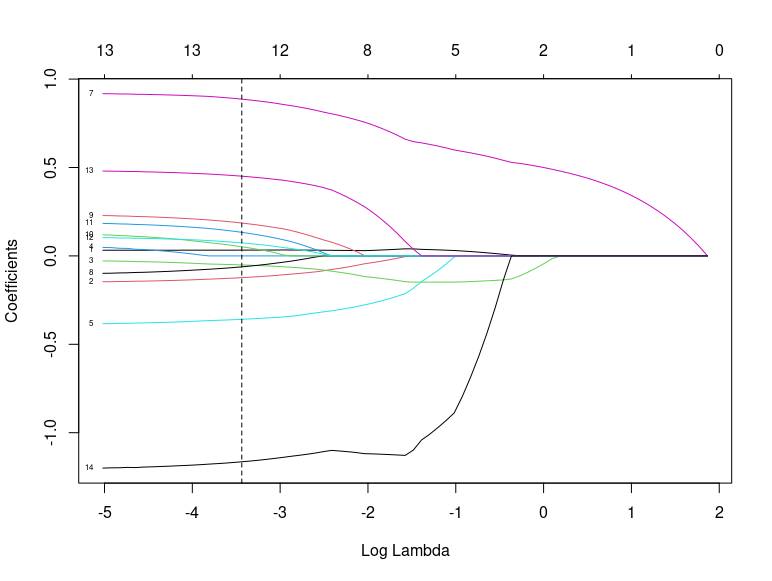
\includegraphics[width=0.7\textwidth]{lasso_path}
  \caption{Path of coefficients vs $\lambda$}
  \label{fig:lasso}
\end{figure}

PCA and PLS regression both transform the dataset in order to perform dimension reduction. In order to find the optimal number of components to include in the final model different stategies were used. For PCA, the total amount of variance each PC explains in the original dataset can be calculated. In order to reduce dimensions but retain as much information, I chose the number of PCs in order to explain at least 95\% of variance. Figure \ref{fig:pca} shows the cumulative explained variance for each additional PC included. It was determined that 8 PCs, were sufficient. 

For PLS, I was able to run a 10-fold cross validation with increasing number of components. The number of components that produced the lowest validation RMSE was 9, which was the selected for the models going forward. Fig \ref{fig:pls} shows the RMSE agains the number of components chosen

\begin{figure}[h!]
  \centering
  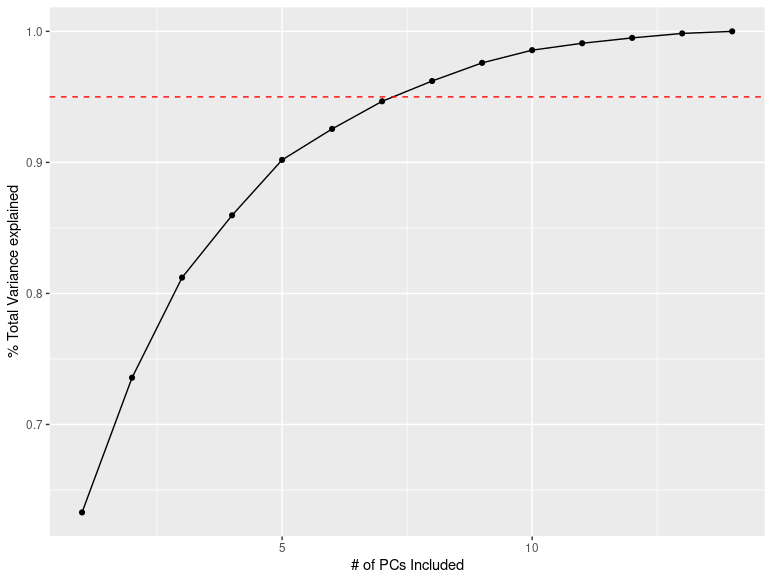
\includegraphics[width=0.5\textwidth]{pca_selection}
  \caption{Cumulative variance explained in PCA components}
  \label{fig:pca}
\end{figure}

\begin{figure}[h!]
  \centering
  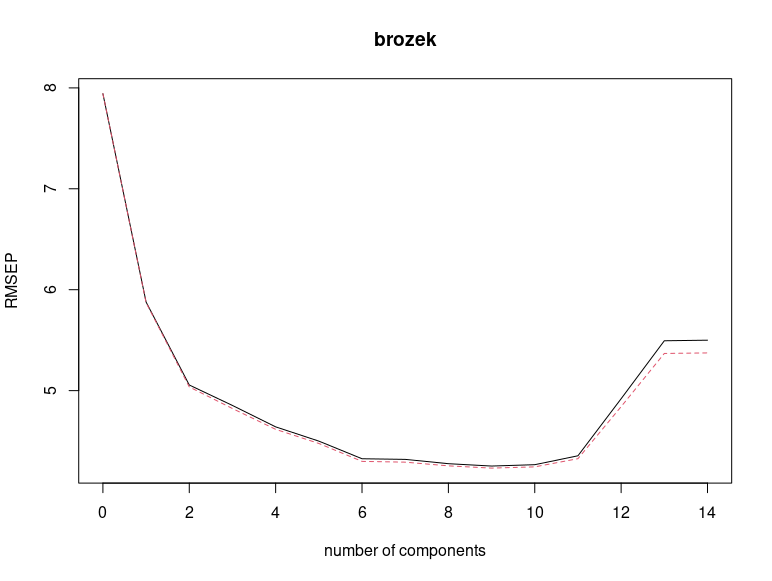
\includegraphics[width=0.5\textwidth]{pls_rmsep}
  \caption{Cross validation results for PLS component selection}
  \label{fig:pls}
\end{figure}

Table \ref{tab:part1} shows the test dataset MSE for each model. The models that removed features entirely tended to perform worse on this test dataset. While removing features can simplify a model, it is expected that some preictive information would be lost in the process. It is also important to note that the test dataset is only 10\% of the total data, which means that the models have a potential to be overfit to the training data.

\begin{table}
  \caption{MSE for each model}
  \centering
  \begin{tabular}[h!]{|l|r|}
  \hline
    & MSE\\
  \hline
  PCA & 9.488612\\
  \hline
  Ridge & 10.174908\\
  \hline
  PLS & 14.141992\\
  \hline
  LASSO & 14.966777\\
  \hline
  Full & 15.015278\\
  \hline
  5-Best (p-score) & 15.457313\\
  \hline
  5-Best (AIC) & 17.021661\\
  \hline
  Stepwise & 17.168963\\
  \hline
  \end{tabular}
  \label{tab:part1}
\end{table}

After 500 MonteCarlo cross validation trials, the mean, median, and stadard deviation of the test errors for each model are shows in Table \ref{tab:mc_cv}. These results are almost completely flipped from part 1. The best models appear to be stepwise regression and the 5-best feature sas chose by AIC. Both have very low mean and median MSE, as well as extremely small deviation. Both methods include AIC in model selection, which tends to favor better predicitive models, which could explain their better performance. The 5-best selected by p-score performing worse solidifies the notion that variable selection by p-score is unreliable since removing features can have a drastic effect on the remaining features p-scores. PLS had a high mean MSE but the lowest median MSE, indicating it was prone to outliers, supported by the high MSE variance. Larger datasets and a higher percentage of test data vs training data might help stabilize some of the results that could be skewed by overfitting. 

It is important to note that the process for fitting each models was repeated for each trial. For example, this means that the 5-best features might be differnet from trial to trial instead of using retaining the model created with the original training dataset. 

\begin{table}

  \caption{Aggregate MSE from 500 MonteCarlo CV Trials}
  \centering
  \begin{tabular}[h]{|l|r|r|r|}
  \hline
    & Mean & Median & Std. Deviation\\
  \hline
  Stepwise & 17.81251 & 17.39974 & 4.86326\\
  \hline
  5-Best (AIC) & 18.12364 & 17.17710 & 5.84921\\
  \hline
  LASSO & 18.61595 & 17.20485 & 11.38024\\
  \hline
  Ridge & 18.96446 & 18.31686 & 5.73992\\
  \hline
  5-Best (p-score) & 19.38463 & 17.75214 & 14.02199\\
  \hline
  PLS & 19.39497 & 17.12886 & 16.47483\\
  \hline
  Full & 20.99267 & 17.60521 & 18.42111\\
  \hline
  PCA & 22.03938 & 21.36599 & 6.89422\\
  \hline
  \end{tabular}
  \label{tab:mc_cv}

\end{table}

\section*{Conclusion}

When creating a linear regression model, it is important to balance a few different factors. Goodness-of-fit and predicitive accuracy are both extremely important. Model complexity is also an important consideration since simpler models are easier to understand and can be worth the trade off. For these reasons, models that employ AIC based feature selection are excellent selections since they balance simplifying a model with retaining it's predictive accuracy. PCA and PLS, while both accomplish dimensional analysis, do not reduce the features needed in the dataset since each new component is a linear combination of all the features. The components are also not easily explained, making them poor choices. Elastic Net, the combination of LASSO and Ridge, is also a good choice for model creation since it can accomplish feature selection while also guarding against collinearity. In concolusion, it is important to attempt a fit different models as well as rigorously cross validate them when creating a linear regression in order to find the model that approriately balances accuracy and simplicity. 

\end{document}